%----------------------------------------------------------------------------------------
%	PACKAGES AND OTHER DOCUMENT CONFIGURATIONS
%----------------------------------------------------------------------------------------

\documentclass[12pt]{article}
\usepackage{polski}
\usepackage[polish]{babel}
\usepackage[utf8]{inputenc}
\usepackage{datetime}
\usepackage{graphicx}
\usepackage[title]{appendix}
\usepackage{listings}
\usepackage{tikz}
\usepackage{amsmath}
\usepackage{multirow}
\usepackage{tabularx}
\usepackage{geometry}
\usepackage{subcaption}
\usepackage{epstopdf}
\usepackage{float}
\usepackage{tabularx}

\geometry{
 	a4paper, 
 	left    = 20mm,
 	right	= 20mm,
 	top     = 20mm,
 	bottom  = 20mm,
}
 
%----------------------------------------------------------------------------------------
 
%----------------------------------------------------------------------------------------
% DATES
%----------------------------------------------------------------------------------------

\renewcommand{\dateseparator}{.}
\newdate{exercise_date}{15}{12}{2016}


% dodatkowe typy kolumn tabel

% flush left fixed width:
\newcolumntype{L}[1]{>{\raggedright\arraybackslash}p{#1}}

% center fixed width:
\newcolumntype{C}[1]{>{\centering\arraybackslash}p{#1}}

% flush right fixed width:
\newcolumntype{R}[1]{>{\raggedleft\arraybackslash}p{#1}}

%----------------------------------------------------------------------------------------

%----------------------------------------------------------------------------------------
% TIKZ PACKAGES
%----------------------------------------------------------------------------------------

\usetikzlibrary{arrows}

%----------------------------------------------------------------------------------------

\begin{document}
  
\begin{titlepage}

\newcommand{\HRule}{\rule{\linewidth}{0.5mm}}
% Defines a new command for the horizontal lines, change thickness here

\center
% Center everything on the page
 
%----------------------------------------------------------------------------------------
%	LOGO SECTION
%----------------------------------------------------------------------------------------


\includegraphics[width=6cm]{img/logo.png}\\[1cm]
% Include a department/university logo - this will require the graphicx package
 
%----------------------------------------------------------------------------------------
 
%----------------------------------------------------------------------------------------
%	HEADING SECTIONS
%----------------------------------------------------------------------------------------

\textsc{\LARGE Akademia Górniczo-Hutnicza \\[0.2cm]
im. Stanisława Staszica w Krakowie}\\[1.5cm]
% Name of your university/college

\textsc{\Large Elektroniczne systemy diagnostyki medycznej i terapii}\\[0.5cm]
% Major heading such as course name

%----------------------------------------------------------------------------------------
%	TITLE SECTION
%----------------------------------------------------------------------------------------

\HRule \\[0.5cm]
{ \huge \bfseries Klasyfikacja sygnału EKG z wykorzystaniem algorytmów kNN i eNN}\\[0.3cm]
% Title of your document
\HRule \\[1.5cm]

\flushright
\Large \emph{Autorzy:}\\
Wojciech \textsc{Gumuła}\\[0.1cm]
Krzysztof \textsc{Mazur}\\[3cm]
% Authors

%----------------------------------------------------------------------------------------
%	DATE SECTION
%----------------------------------------------------------------------------------------
% Data wykonania ćwiczenia: \\
%{\large \displaydate{exercise_date}}\\[1cm]


\vfill % Fill the rest of the page with whitespace

\end{titlepage}
\tableofcontents

%%\large{
\pagebreak
\section*{Abstrakt}

Celem projektu było zbadanie możliwości wykorzystania algorytmu k-Nearest Neighbours oraz jego rozszerzonej wersji w zadaniu klasyfikacji zespołów \textit{QRS} sygnału \textit{EKG}. Metoda \textit{kNN} charakteryzuje się stosunkowo niewielką złożonością obliczeniową i prostotą implementacji, oferując przy tym klasyfikację z dużą dokładnością. Rozszerzona metoda \textit{eNN} pozwala na uwzględnienie otoczenia klasyfikowanego wektora, co może zwiększyć dokładność wyniku. W ramach projektu przygotowano prototyp algorytmów w środowisku Matlab oraz ich implementację w języku C++ przy użyciu biblioteki Eigen.


\textbf{Słowa kluczowe}:
EKG, QRS, kNN, eNN, klasyfikacja, rozpoznawanie wzorców, Matlab, Eigen.
\chapter{Wprowadzenie}
Badanie elektrokardiograficzne, dzięki swej dostępności i łatwości wykonania stanowi jedno z najczęściej wykorzystywanych metod rozpoznawania zaburzeń w pracy serca. Uzyskiwany przy jego pomocy sygnał EKG dostarcza informacji o elektrycznej aktywności mięśnia sercowego, jako różnicę potencjałów pomiędzy dwoma elektrodami.

Jednym z najbardziej charakterystycznych elementów typowego sygnału EKG są zespoły QRS. Jest to układ trzech załamków opisujących proces depolaryzacji mięśnia. Ideowy schemat EKG, wraz z kompleksem QRS przedstawiono na rysunku \ref{fig:qrs-complex}.


\begin{figure}[H]
	\centering
	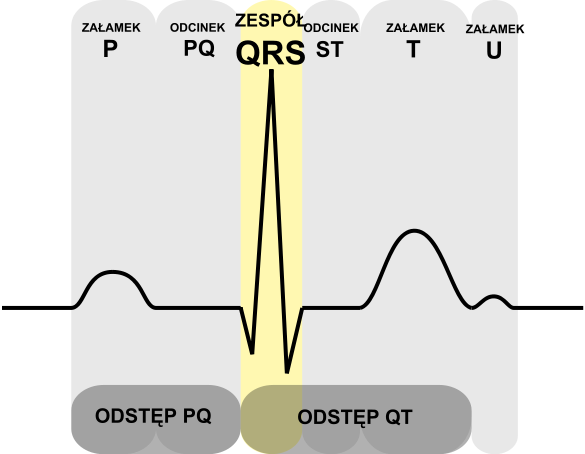
\includegraphics[width=8cm]{img/qrs-complex}
	\caption{Ideowy schemat sygnału EKG. Źródło: \cite{qrs-wiki}}
	\label{fig:qrs-complex}
\end{figure}

Na podstawie charakteru zespołu QRS diagnozować można szereg dysfunkcji serca. Wykorzystanie w tym celu zautomatyzowanych procedur diagnostycznych pozwala na zwiększenie prawdopodobieństwa wykrycia nieprawidłowości i przyśpiesza proces badania. Wymaga to jednak wyodrębnienia grup kompleksów o podobnych parametrów. Uzyskane grupy powinny w odwzorowywać najczęściej występujące zaburzenia pracy.

\section{Koncepcja proponowanego rozwiązanie}

Autorzy badali możliwość wykorzystania algorytmu kNN (\textit{k Nearest Neighbours}) oraz jego rozszerzonej wersji, eNN (\textit{extended Nearest Neighbours}) do zaprojektowania zautomatyzowanego procesu klasyfikacji zespołów QRS do predefiniowanych grup. Opis algorytmów przedstawiono w rozdziałach \ref{chap:knn} i \ref{chap:enn}.

Metody klasy \textit{NN} wymagają przedstawienia danych wejściowych w postaci wektora cech o ustalonym wymiarze. Zdecydowano się wykorzystać w tym celu dane dostępne w opracowaniu \cite{heart-class-module}. Uwzględniono przy tym klasyfikację w zbiorze trzech klas, zaproponowaną przez autorów, a także w zbiorze uwzględniającym wszystkie klasy definiowane w dokumentacji bazy \textit{MIT-BIH} \cite{mitdb}.

Dane wejściowe opisywane są wektorem składającym się z osiemnastu cech. Wektor zawiera informacje na temat chwil wystąpienia kolejnych elementów kompleksu QRS a także wartości sygnału w istotnych chwilach. Jedna z kolumn - chwila wystąpienia załamka R - związana jest jednoznacznie z badanym sygnałem EKG i nie pozwala na klasyfikację w uogólnionym zbiorze danych, z tego powodu jest ignorowana w zaprojektowanym rozwiązaniu.

Celem projektu było zaprojektowanie prototypu proponowanego rozwiązania przy użyciu oprogramowania \textit{Matlab}, a także zgodnej z nim implementacji w języku \textit{C++}. Wykorzystano również bibliotekę \textit{Eigen} \cite{eigen-www}, pozwalającą na optymalizację operacji matematycznych na macierzach i wektorach.

Cykl działania aplikacji podzielić można na dwa etapy.
\begin{enumerate}
	\item Proces uczenia.
	
	Program uczony jest przy użyciu wybranego zbioru danych wejściowych wraz z poprawną klasyfikacją każdego wektora. Dane te są zapamiętywane i wykorzystywane w kolejnym etapie pracy.
	
	\item
	Klasyfikacja danych wejściowych.
	
	Aplikacja pozwala na klasyfikację dowolnej liczby wektorów danych, porównując je z posiadanym zbiorem referencyjnym. Wyjściem programu na wejście zawierające jeden wektor testowy jest klasa, do której został on przypisany.
\end{enumerate}

Test poprawności działania implementacji wymagał podzielenia znanego zbioru danych na podzbiory - uczący i testowy, wraz ze związanymi z nimi klasami. Przyjęto podział w stosunku dwa do jednego. Działanie algorytmu badane było niezależnie dla każdego pliku wejściowego.

\section{Dane wejściowe}
Na etapie testowania działania proponowanych algorytmów wykorzystano dane zgromadzone w ramach biblioteki arytmii pracy serca \textit{MIT-BIH}. Zbiór zawiera czterdzieści osiem zapisów trzydziestominutowych badań \textit{EKG}. Dwadzieścia trzy nagrania stanowią losowo wybrany podzbiór bazy zawierającej zapis kilku tysięcy badań, natomiast pozostałe dwadzieścia pięć nagrań to zbiór dobrany w taki sposób, by zawierał istotne lecz rzadziej występujące klasy arytmii. Dane zawarte w bazie zawierają również precyzyjną klasyfikację kompleksów \textit{QRS} dla każdego nagrania.

Dane zawarte w bazie danych nie mogą być bezpośrednio wykorzystane do przeprowadzenia procesu klasyfikacji. Sygnał wejściowy musi zostać poddany filtracji oraz ograniczony do wektorów cech opisujących kolejne zespoły \textit{QRS}. W ramach projektu wykorzystano wstępnie przygotowane dane wejściowe, zawierające wektory cech i adnotacje klas.

Wykorzystując opisany zbiór wejściowy, badano skuteczność detekcji klas przez algorytm. Sprawdzano również możliwość zaprojektowania zbioru uczącego w taki sposób, aby jak najlepiej reprezentował on klasy sygnału, maksymalizując skuteczność detekcji w zbiorze zawierającym wszystkie pliki danych.
\section{Algorytm kNN}
\label{chap:knn}
Algorytm kNN (ang. \textit{k Nearest Neighbours})  jest jednym z najprostszych algorytmów klasyfikacyjnych, należy również do najpopularniejszych ze względu na prostotę implementacji oraz dobre wyniki obliczeń. Reguła klasyfikacji opiera się na założeniu, że dane przedstawione w $n$-wymiarowej przestrzeni zgrupowane będą w obszarach opisanych podobnymi cechami. Bazując na tym założeniu, ustalenie klasy dla wektora wejściowego sprowadza się do zbadania jego najbliższego otoczenia w przestrzeni i wyboru klasy najczęściej w nim występującej.

Pierwszym krokiem algorytmu jest wyznaczenie odległości pomiędzy próbką ze zbioru testowego, oraz wszystkimi próbkami ze zbioru uczącego. Najczęściej stosowaną metodą wyznaczania odległości jest metryka euklidesowa dana poniższym wzorem, gdzie $N$ to szerokość wektora dla każdej próbki:

\begin{equation}
d(x,y) = \sum_{i=1}^{N} \sqrt{(x_i - y_i)^2}.
\end{equation}

Następnie ze zbioru $K$ najbliższych sąsiadów wybierana jest najczęściej występująca klasa obiektów, a rozważany przypadek klasyfikowany jest jako obiekt tej klasy. Dobór optymalnego parametru $K$ odbywa się zazwyczaj na drodze eksperymentów stosując nieparzyste wartości $K=1,3,5...$ . Proces uczenia jest bardzo prosty i ogranicza się do zapamiętania wszystkich próbek ze zbioru uczącego. Konieczność wyznaczenia odległości pomiędzy klasyfikowaną próbką a wszystkimi próbkami ze zbioru uczącego wymusza rozważne przygotowanie tego ostatniego. Zawarte w nim wartości powinny dobrze definiować całą przestrzeń, jednocześnie minimalizując rozmiar w celu przyspieszenia działania algorytmu. Poza klasyfikacją algorytm kNN wykorzystywany jest także do klasteryzacji, regresji, estymowania funkcji gęstości. W 2006 roku algorytm został zaliczony do 10 najpopularniejszych algorytmów w dziedzinie eksploracji danych podczas konferencji IEEE w Hong Kongu.

Zasadę działania algorytmu na przykładzie przedstawiono na rysunku \ref{fig:knn-idea}.

\begin{figure}[H]
	\centering
	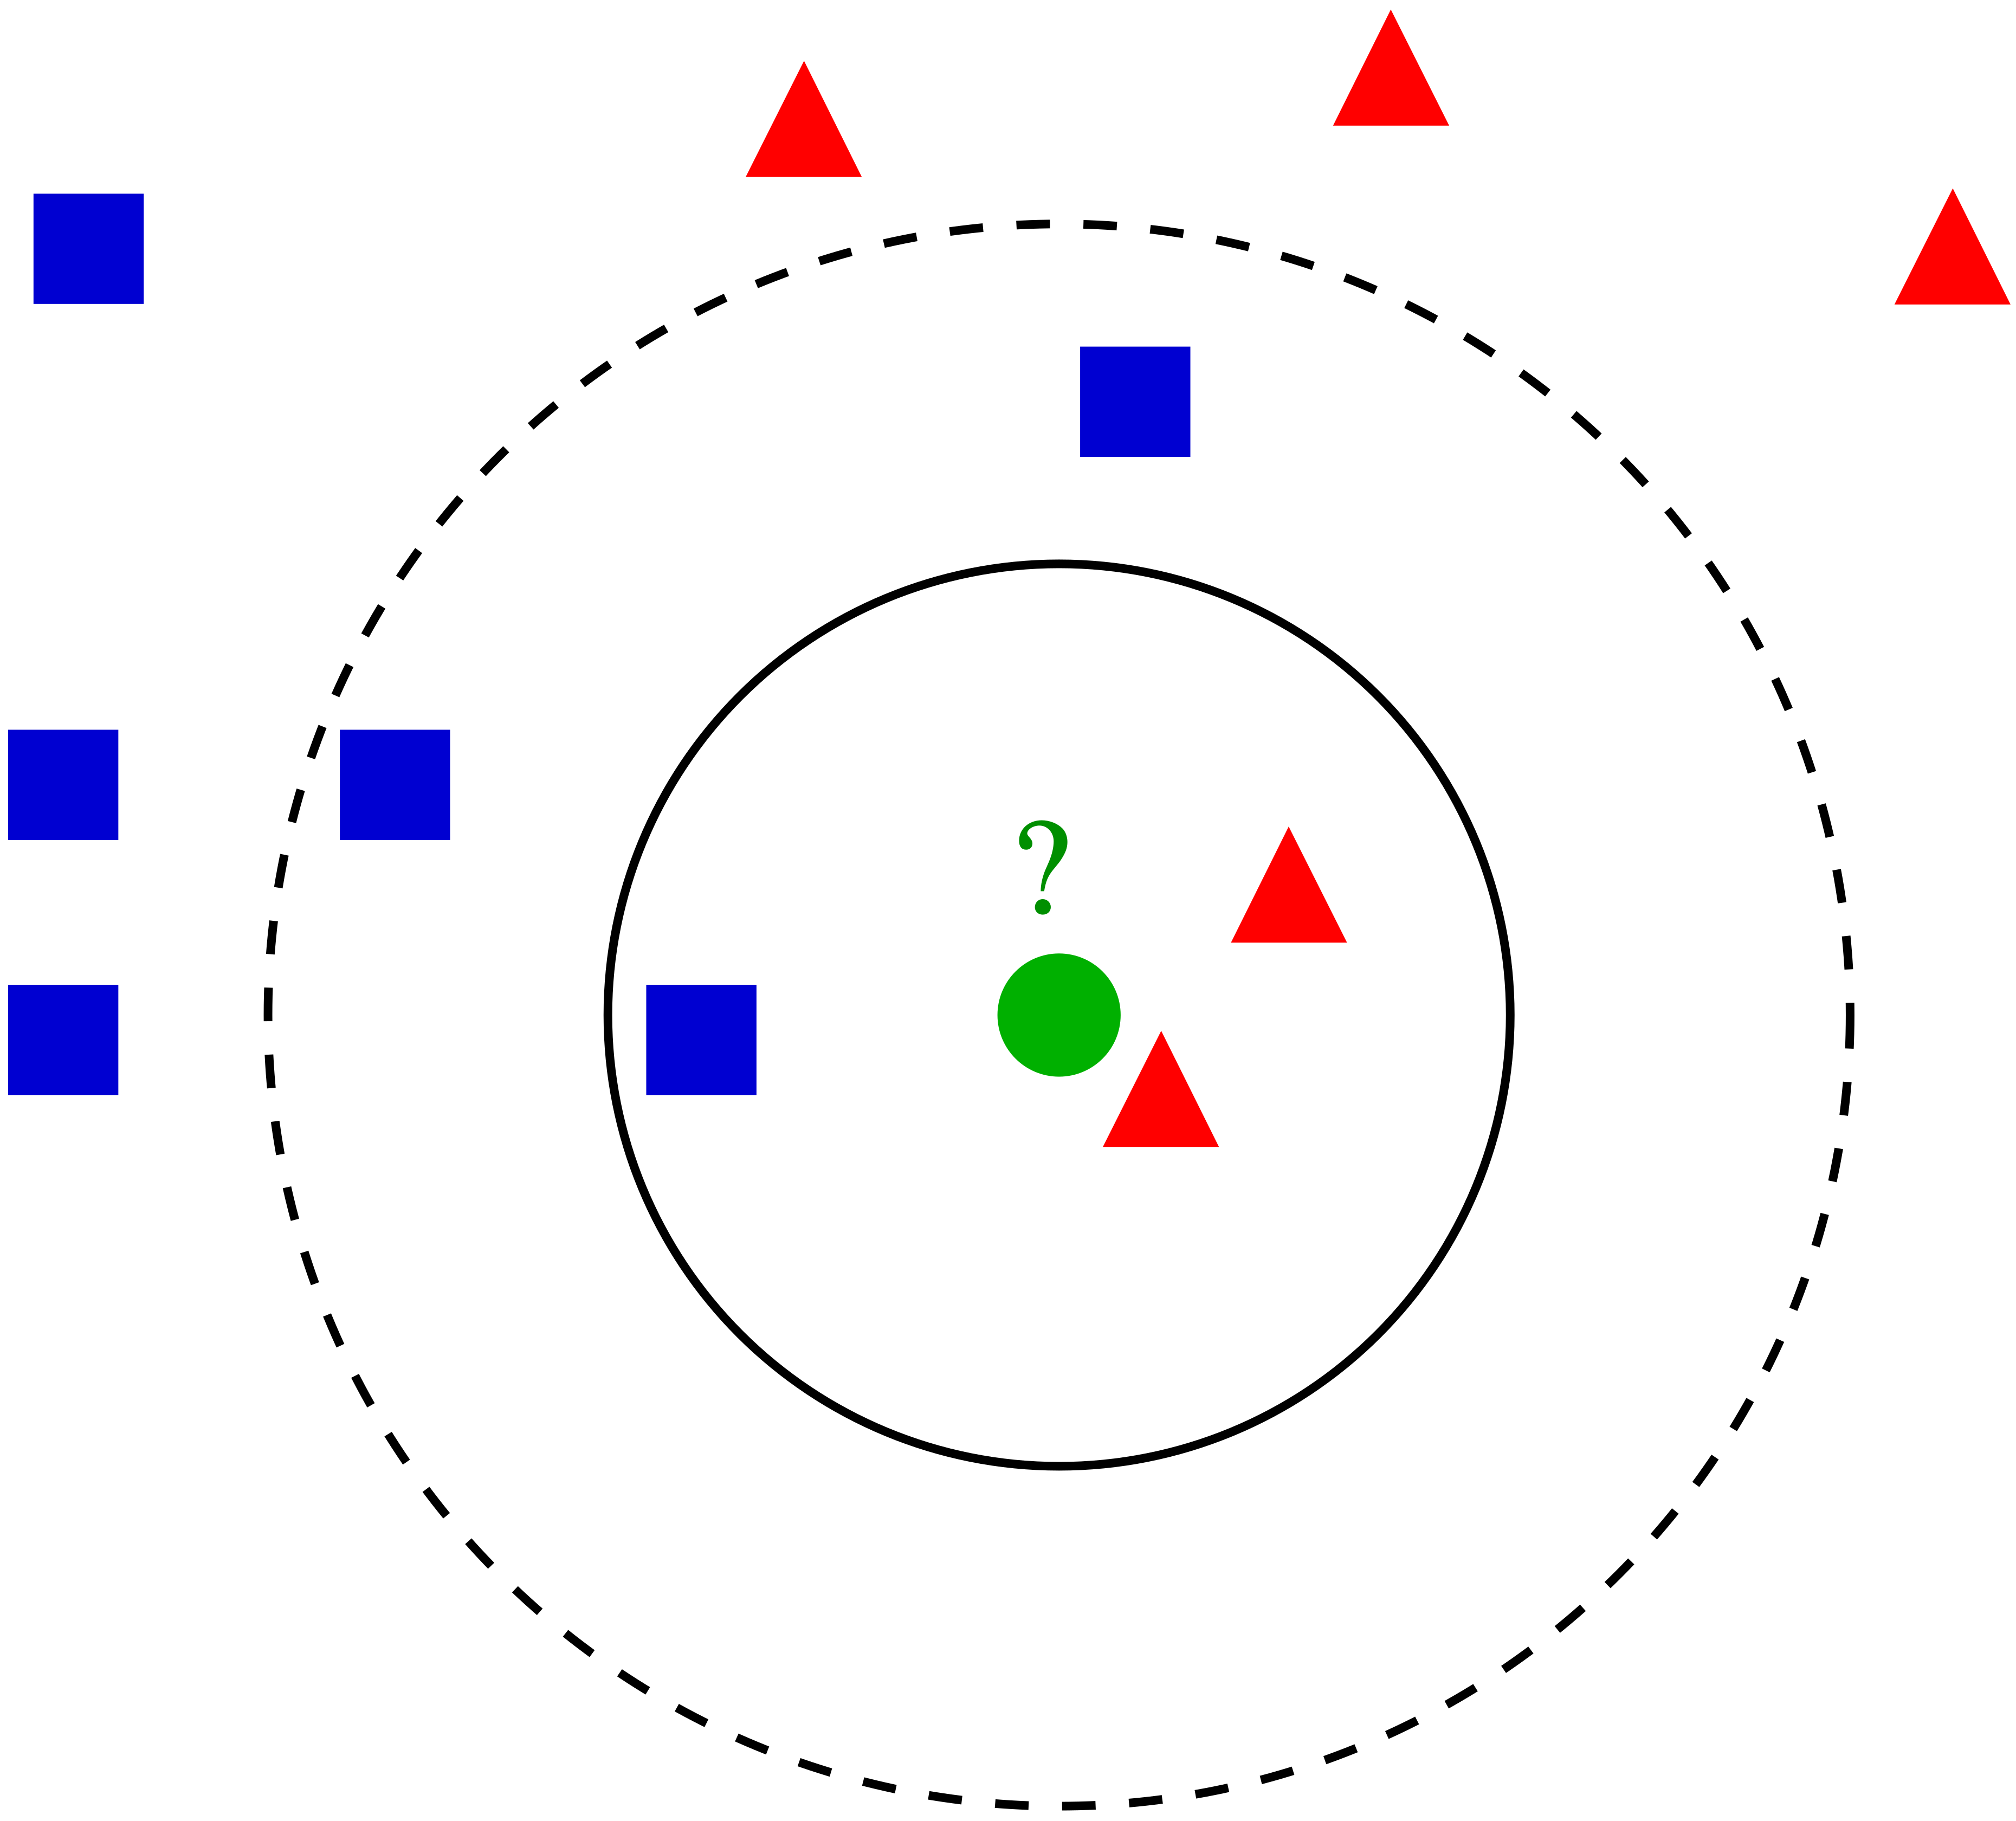
\includegraphics[width=10cm]{img/KnnClassification}
	\caption{Schematyczne przedstawienie klasyfikacji dwuwymiarowego wektora danych. Źródło \cite{knn-wiki}}
	\label{fig:knn-idea}
\end{figure}

Zadaniem klasyfikacji jest ustalenie przynależności wartości wejściowej - koła, do jednej z dwóch grup elementów - kwadratów i trójkątów. Przyjmując wartość parametru $K=3$ (linia ciągła na rysunku), wartość przypisana zostanie do grupy zawierającej trójkąty. Zakładając $K=5$ wynik będzie przeciwny i element zostanie powiązany z grupą zawierającą kwadraty.

Dobór wartości parametru $K$ dającej najlepsze wyniki wymaga więc znajomości badanego zjawiska bądź przeprowadzenia doświadczeń na reprezentatywnym zbiorze testowym.

\chapter{Algorytm eNN}
\label{chap:enn}
\section{Podstawowa wersja algorytmu}
\large{Algorytm kNN pomimo wielu swoich zalet ma także kilka wad, które w niektórych przypadkach mogą niekorzystnie wpływać na wyniki działania. Jednym z charakterystycznych problemów jest przypadek kiedy rozkłady gęstości poszczególnych klas nie są równe. W takiej sytuacji elementy klasy o większym rozkładzie gęstości przeważają nad elementami pozostałych klas na danym obszarze. Dla algorytmu większość najbliższych sąsiadów będzie pochodziła z dominującej klasy co może zakłócać poprawność działania.

Jako rozwinięcie algorytmu kNN został stworzony algorytm eNN (\textit{ang. Extended Nearest Neighbours}) \cite{haibo-he}. Zaproponowana metoda podczas klasyfikacji bierze pod uwagę nie tylko k najbliższych sąsiadów klasyfikowanego obiektu, ale również ich otoczenie. 

Dla uproszczenia opis algorytmu zostanie przeprowadzony dla przypadku klasyfikacji pomiędzy dwoma klasami. Uogólnienie algorytmu dla dowolnej ilości klas sprowadza się jedynie do większej złożoności obliczeniowej. Dla każdego z k najbliższych sąsiadów próbki ze zbioru testowego wyznaczana jest funkcja statystyczna T opisująca otoczenie w jakim się znajduje. Funkcja T wyznaczana jest według wzoru:

\begin{equation}
T_{i} = \frac{1}{n_i k} {\sum_{x \in S_i} \sum_{r=1}^{k} I_r (x,S \in (S_1 \cup S_2))} 
\end{equation}\\
gdzie $S_1$ i $S_2$ są zbiorami próbek należących odpowiednio do klas 1 i 2, k jest zdefiniowaną ilością najbliższych sąsiadów a $I_r$ dane jest wzorem:

\begin{equation}
I_r(x,S) =\left\{\begin{matrix}
1 &&	dla\ x \in S_i \wedge NN_{r}(x,S) \in S_i
\\
0 &&	w\ pozostałych\ przypadkach
\end{matrix}\right.
\end{equation}
Funkcja $I_r$ przyjmuje wartość 1 jeżeli próbka x i jej r-sąsiad należą do tej samej klasy, natomiast wartość 0 przyjmuje w pozostałych przypadkach.
Funkcja $T_i$ przyjmuje wartości z zakresu [0,1]. Im większa wartość $T_i$ tym więcej próbek tej samej klasy znajduje się w otoczeniu badanej próbki. Małe wartości oznaczają małą ilość próbek tej samej klasy.

Mając nową, niesklasyfikowaną próbkę, w kolejnych krokach zostaje przypisana do poszczególnych klas a następnie dla każdego przypadku wyznaczona zostaje wartość funkcji $T_i^j$ według wzoru:

\begin{equation}
T_{i}^{j} = \frac{1}{n_i^j k} {\sum_{x \in S_{i,j}'} \sum_{r=1}^{k} I_r (x,S' \in (S_1 \cup S_2 \cup {Z}))} 
\end{equation}\\
gdzie j oznacza klasę do której została przypisana próbka Z.
W rozważanym przypadku, gdy pod uwagę brane są dwie klasy otrzymujemy cztery wyniki $T_1^1, T_2^1, T_1^2\ oraz\ T_2^2$. Próbka Z zostaje zakwalifikowana zgodnie ze wzorem:

\begin{equation}
f_{ENN} = arg_{j\in1,2} max \sum_{i=1}^{2} T_i^j
\end{equation}
Powyższy wzór w przypadku gdy w zbiorze znajduje się N klas występuje w postaci:
\begin{equation}
f_{ENN} = arg_{j\in1,2,..,N} max \sum_{i=1}^{N} T_i^j
\end{equation}
Klasyfikacja próbki do odpowiedniej klasy odbywa się poprzez wybór maksymalnej wartości funkcji $T_i$ spośród wyznaczonych metodą iteracyjną wartości dla kolejnych klas.

\newpage
\section{Alternatywna wersja algorytmu}
Analizując podstawową wersję algorytmu eNN można zaobserwować konieczność wyznaczenia wartości $T_i^j$ dla każdej kolejnej klasyfikowanej próbki. Wiąże się to  ze wzrostem złożoności obliczeniowej co nie jest pożądane w przypadku dużych zbiorów testowych. Rozwiązaniem tego problemu jest równoważna wersja algorytmu eNN, która została przedstawiona w tym paragrafie. 

W rozważanej wersji algorytmu pod uwagę brane jest nie tylko kto znajduje się w zbiorze najbliższych sąsiadów klasyfikowanej próbki Z ale także które próbki ze zbioru uczącego biorą pod uwagę próbkę Z jako jednego z k najbliższych sąsiadów. W tym celu próbka Z zostaje przypisana kolejno do wszystkich klas. W każdym przypadku zostają wyznaczone wartości $\Delta n_i^j$ gdzie j jest klasą do której została przypisana próbka Z, natomiast i jest klasą dla której obliczana jest zmiana ilości sąsiadów tej samej klasy. W przypadku gdy i = j zliczana jest ilość próbek klasy i dla której wzrosła ilość sąsiadów należących do tej samej klasy. W przypadku gdy $i\ \neq j$ wyznaczana jest ilość próbek klasy i dla których zmalała ilość sąsiadów należących do tej samej klasy.

Dla wyznaczonych wartości $n_i^j$ klasyfikacja próbki Z realizowana jest zgodnie z zależnością:

\begin{equation}
f_{ENN} = arg_{j \in 1,2,..,N} max \begin{Bmatrix}
(\frac{\Delta n_i^j + k_j -kT_i}{(n_i+1)k})
\end{Bmatrix}_{i=j} - \sum_{i \neq j}^N \frac{\Delta n_i^j}{n_i k}
\end{equation}\\
gdzie k jest zdefiniowaną ilością najbliższych sąsiadów, $n_i$ jest ilością próbek należących do klasy i, a $k_i$ jest ilością najbliższych sąsiadów należących do klasy i.

Obie wersje algorytmu są równoważne, jednak w przypadku drugiej wersji na początku działania algorytmu można wyznaczyć wektor wartości $T_i$ a podczas klasyfikacji kolejnych próbek ograniczyć się do wyznaczenia zmian w otoczeniach k najbliższych sąsiadów próbki Z, dla kolejnych przypisań próbki Z do odpowiednich klas.

\section{Prototyp algorytmu}
Po zapoznaniu z wiadomościami teoretycznymi i ustaleniu zakresu projektu, przystąpiono do zaprojektowania prototypów algorytmów $kNN$ oraz $eNN$ w środowisku Matlab.

Algorytm badany był przy użyciu zbioru sygnałów $EKG$ zredukowanych do opisu cech zespołów $QRS$, uporządkowanych do zbioru trzech klas. Pierwsza klasa oznaczała normalny zespół QRS lub atyrmię nadkomorową, klasa druga arytmię komorową, natomiast klasa trzecia zawierała nierozpoznane próbki. 

Dane wejściowe poddano normalizacji, która opisana jest równaniem \ref{eq:normalize-data}.

\begin{equation}
\label{eq:normalize-data}
x_j = \frac{x_j - \mu(x_j)}{\sigma(x_j)}, j=1,2...N
\end{equation}
gdzie $x_j$ opisuje $j$-tą kolumnę macierzy danych.

Skuteczność badano niezależnie dla każdego pliku. Wyniki przedstawiono w tabeli \ref{tab:matlab-skutecznosc}. Przyjęto $K=3$. Zmierzono również czas wykonania algorytmów dla wszystkich plików.

\begin{table}[H]
	\centering
	\begin{tabular}{|c|r|r|r|r|}
		\hline
		& \multicolumn{2}{c|}{$kNN$} & \multicolumn{2}{c|}{$eNN$} \\
		\hline
		$Plik$ & Skuteczność & Czas wykonania [s] & Skuteczność & Czas wykonania [s] \\
		\hline
100 &  98.02\% & 0.1658 &  88.11\% & 0.4700 \\ 
\hline
101 &  96.78\% & 0.1061 &  94.85\% & 0.2958 \\ 
\hline
102 &  98.07\% & 0.1356 &  92.56\% & 0.3935 \\ 
\hline
103 &  98.27\% & 0.1246 &  87.88\% & 0.3563 \\ 
\hline
104 &  98.16\% & 0.1287 &  88.97\% & 0.3740 \\ 
\hline
105 &  97.87\% & 0.1823 &  88.86\% & 0.5248 \\ 
\hline
106 &  98.86\% & 0.0989 &  83.85\% & 0.2724 \\ 
\hline
107 &  98.47\% & 0.0939 &  90.85\% & 0.2619 \\ 
\hline
108 &  96.71\% & 0.0677 &  85.83\% & 0.1887 \\ 
\hline
109 &  97.87\% & 0.1638 &  88.60\% & 0.4717 \\ 
\hline
111 &  98.63\% & 0.1130 &  90.29\% & 0.3206 \\ 
\hline
112 &  97.99\% & 0.1813 &  92.79\% & 0.5302 \\ 
\hline
113 &  98.16\% & 0.0960 &  88.29\% & 0.2647 \\ 
\hline
114 &  97.44\% & 0.0321 &  86.54\% & 0.0843 \\ 
\hline
115 &  98.77\% & 0.1087 &  86.33\% & 0.3057 \\ 
\hline
117 &  96.59\% & 0.0707 &  87.78\% & 0.1948 \\ 
\hline
118 &  98.12\% & 0.1406 &  88.74\% & 0.4063 \\ 
\hline
119 &  99.24\% & 0.1129 &  91.24\% & 0.3151 \\ 
\hline
121 &  97.58\% & 0.1028 &  80.65\% & 0.2823 \\ 
\hline
122 &  97.58\% & 0.1737 &  87.15\% & 0.5027 \\ 
\hline
123 &  96.82\% & 0.0713 &  87.67\% & 0.1973 \\ 
\hline
124 &  96.73\% & 0.0694 &  87.35\% & 0.1901 \\ 
\hline
200 &  99.10\% & 0.1163 &  82.88\% & 0.3250 \\ 
\hline
201 &  96.60\% & 0.0854 &  92.67\% & 0.2503 \\ 
\hline
202 &  97.58\% & 0.1271 &  89.90\% & 0.3596 \\ 
\hline
203 &  97.89\% & 0.1660 &  87.48\% & 0.4783 \\ 
\hline
205 &  98.03\% & 0.1892 &  97.10\% & 0.5376 \\ 
\hline
208 &  98.12\% & 0.2058 &  92.03\% & 0.5999 \\ 
\hline
209 &  97.88\% & 0.2533 &  89.42\% & 0.7110 \\ 
\hline
210 &  97.91\% & 0.1686 &  92.99\% & 0.4871 \\ 
\hline
212 &  97.81\% & 0.2062 &  88.40\% & 0.6042 \\ 
\hline
213 &  98.51\% & 0.2764 &  85.89\% & 0.8126 \\ 
\hline
214 &  99.11\% & 0.1176 &  88.28\% & 0.3398 \\ 
\hline
215 &  98.10\% & 0.2922 &  88.95\% & 0.8516 \\ 
\hline
217 &  99.39\% & 0.1138 &  84.24\% & 0.3163 \\ 
\hline
219 &  98.32\% & 0.1313 &  89.09\% & 0.3745 \\ 
\hline
220 &  98.68\% & 0.1172 &  92.82\% & 0.3367 \\ 
\hline
221 &  97.74\% & 0.1638 &  85.03\% & 0.4674 \\ 
\hline
222 &  97.42\% & 0.1672 &  85.40\% & 0.4860 \\ 
\hline
223 &  97.59\% & 0.1601 &  86.08\% & 0.4525 \\ 
\hline
228 &  98.14\% & 0.0919 &  92.05\% & 0.2574 \\ 
\hline
230 &  97.73\% & 0.1259 &  84.96\% & 0.3714 \\ 
\hline
231 &  97.30\% & 0.0869 &  90.56\% & 0.2352 \\ 
\hline
232 &  98.13\% & 0.0949 &  85.20\% & 0.2727 \\ 
\hline
233 &  98.03\% & 0.1922 &  89.55\% & 0.5452 \\ 
\hline
234 &  98.03\% & 0.2122 &  92.25\% & 0.6151 \\ 
\hline
		
	\end{tabular}
	\caption{Wyniki pracy algorytmu kNN i eNN w środowisku Matlab.}
	\label{tab:matlab-skutecznosc}
	
\end{table}

Wyniki otrzymane za pomocą algorytmów $kNN$ oraz $eNN$ są zbliżone do siebie z lekką przewagą algorytmu $kNN$. Duży wpływ na działanie algorytmów miał podział próbek w zbiorze uczącym na poszczególne klasy. Znaczna przewaga danych należących do klasy 1 miała negatywny wpływ na skuteczność klasyfikacji, co jest uzasadnione w przypadku korzystania z metod statystycznych. W optymalnie przygotowanym zbiorze uczącym próbki powinny być równomiernie rozłożone na wszystkie klasy. Czas wykonania algorytmu $eNN$ jest zwykle około trzykrotnie dłuższy niż w przypadku algorytmu $kNN$. Bardzo ważne okazało się zastosowanie obliczeń wektorowych, które są bardzo dobrze zoptymalizowane w środowisku Matlab i cechują się znacznie większą wydajnością niż podejście iteracyjne. W przypadku algorytmu $eNN$ różnice w czasie obliczeń przekraczały trzy rzędy wielkości.
\section{Implementacja w języku C++}
\subsection{Proces projektowania}
Cechy środowiska Matlab ułatwiają przeprowadzenie procesu prototypowania i wstępnego testowania aplikacji, co jednak nie jest równoznaczne aspektom koniecznym do zaprojektowania możliwie najwydajniejszej i stabilnej aplikacji klasyfikującej sygnał $EKG$. Z tego względu, po zakończeniu procesu prototypowania zaprojektowano program w języku C++, wykorzystujący badane algorytmy. W trakcie pracy wykorzystano bibliotekę $Eigen$, oferującą wydajną implementację operacji arytmetycznych na macierzach. Użyto również biblioteki $IGL$ \cite{libigl-www}, oferującej szereg funkcji dostępnych w środowisku Matlab oraz interfejsu $OpenMP$ \cite{openmp-www}, umożliwiającego tworzenie programów wykorzystujących zalety systemów wieloprocesorowych.

Zaprojektowany program był w pełni kompatybilny z przygotowanymi prototypami algorytmów, wyniki klasyfikacji oraz cechy nie odbiegały od danych uzyskanych w środowisku Matlab. Dzięki zrównolegleniu sekcji odpowiedzialnych za klasyfikację wektorów testowych osiągnięto kilkukrotnie większą wydajność względem prototypu. Wyniki zebrano w tabeli \ref{matlab-vs-cpp-time}.

\begin{table}[H]
	\centering
	\begin{tabular}{|c|r|r|r|r|}
		\hline
		Plik & KNN Matlab & KNN C++ & ENN Matlab & ENN C++  \\ 
\hline
$100$ & 0.0530 & 0.0203 & 0.1356 & 0.0329 \\
\hline
$101$ & 0.0175 & 0.0109 & 0.0572 & 0.0141 \\
\hline
$102$ & 0.0164 & 0.0109 & 0.0489 & 0.0095 \\
\hline
$103$ & 0.0161 & 0.0084 & 0.0617 & 0.0097 \\
\hline
$104$ & 0.0072 & 0.0035 & 0.0265 & 0.0043 \\
\hline
$105$ & 0.0837 & 0.0227 & 0.2662 & 0.0557 \\
\hline
$106$ & 0.0385 & 0.0119 & 0.1135 & 0.0218 \\
\hline
$108$ & 0.0015 & 0.0013 & 0.0072 & 0.0015 \\
\hline
$109$ & 0.0123 & 0.0059 & 0.0351 & 0.0087 \\
\hline
$111$ & 0.0064 & 0.0039 & 0.0148 & 0.0051 \\
\hline
$112$ & 0.0906 & 0.0298 & 0.2721 & 0.0691 \\
\hline
$113$ & 0.0213 & 0.0083 & 0.0616 & 0.0134 \\
\hline
$118$ & 0.0015 & 0.0019 & 0.0041 & 0.0014 \\
\hline
$119$ & 0.0265 & 0.0090 & 0.0771 & 0.0148 \\
\hline
$121$ & 0.0163 & 0.0067 & 0.0413 & 0.0099 \\
\hline
$122$ & 0.0631 & 0.0169 & 0.1756 & 0.0380 \\
\hline
$124$ & 0.0225 & 0.0075 & 0.0656 & 0.0119 \\
\hline
$200$ & 0.0049 & 0.0028 & 0.0107 & 0.0032 \\
\hline
$201$ & 0.0021 & 0.0012 & 0.0041 & 0.0013 \\
\hline
$202$ & 0.0127 & 0.0056 & 0.0332 & 0.0078 \\
\hline
$203$ & 0.0434 & 0.0137 & 0.1157 & 0.0243 \\
\hline
$205$ & 0.0577 & 0.0180 & 0.1771 & 0.0394 \\
\hline
$208$ & 0.0272 & 0.0100 & 0.0850 & 0.0264 \\
\hline
$209$ & 0.0073 & 0.0043 & 0.0173 & 0.0055 \\
\hline
$210$ & 0.0941 & 0.0274 & 0.3368 & 0.0713 \\
\hline
$212$ & 0.0159 & 0.0068 & 0.0433 & 0.0101 \\
\hline
$213$ & 0.1775 & 0.0439 & 0.5610 & 0.1048 \\
\hline
$214$ & 0.0064 & 0.0042 & 0.0166 & 0.0051 \\
\hline
$215$ & 0.0137 & 0.0064 & 0.0366 & 0.0097 \\
\hline
$217$ & 0.0033 & 0.0026 & 0.0082 & 0.0030 \\
\hline
$219$ & 0.0548 & 0.0210 & 0.1791 & 0.0352 \\
\hline
$221$ & 0.0084 & 0.0046 & 0.0234 & 0.0062 \\
\hline
$222$ & 0.0602 & 0.0174 & 0.1918 & 0.0350 \\
\hline
$223$ & 0.0015 & 0.0014 & 0.0050 & 0.0015 \\
\hline
$228$ & 0.0359 & 0.0117 & 0.1099 & 0.0230 \\
\hline
$231$ & 0.0522 & 0.0157 & 0.1629 & 0.0304 \\
\hline
$233$ & 0.0490 & 0.0159 & 0.1503 & 0.0332 \\
\hline
$234$ & 0.1096 & 0.0310 & 0.3523 & 0.0702 \\
\hline	
	\end{tabular}
	\caption{Porównanie czasu działania w sekundach dla algorytmów zaprojektowanych w Matlabie i C++.}
	\label{tab:matlab-vs-cpp-time}	
\end{table}
Algorytm $KNN$ zaprojektowany w języku C++ wykonywał się średnio $2.45$ razy szybciej od prototypu w Matlabie, natomiast algorytm $ENN$ - średnio $4.38$ razy szybciej. $ENN$ wymaga ponadto średnio o $76\%$ więcej czasu od $KNN$ na przeprowadzenie obliczeń dla tego samego zbioru danych.

\subsection{Wpływ rozmiaru badanych zbiorów na wydajność aplikacji}
Algorytm $KNN$ wymaga analizy pełnego zbioru uczącego dla każdego badanego wektora. Czas wykonania aplikacji zależy więc w sposób liniowy zarówno od rozmiaru obu zbiorów. W przypadku analizy danych poprzez podział zbioru na zbiór uczący i testowy ze stałym współczynnikiem, czas potrzebny na przeprowadzenie obliczeń zależy kwadratowo od wielkości zbioru wejściowego.

Proces uczenia w przypadku algorytmu $ENN$ wymaga przeprowadzenia obliczeń zależnych liniowo od wielkości zbioru uczącego oraz liczby unikalnych klas. Czas wymagany do przeprowadzenia klasyfikacji zależy liniowo od liczności zbioru testowego oraz liczby wektorów uczących.

Złożoność obliczeniowa obu algorytmów zdominowana jest przez wielkość zbiorów uczącego i testowego. Na etapie testowania aplikacji założono, że relacja pomiędzy wielkością zbiorów jest stała. Czasowa złożoność obliczeniowa w takim przypadku opisana być może pewną funkcją kwadratową, której argumentem jest wielkość zbioru na wejściu aplikacji.
Na rysunkach \ref{fig:knn_compexity} i \ref{fig:enn_complexity} przedstawiono dane eksperymentalne z działania algorytmów na zbiorach różnych rozmiarów.

\begin{figure}[H]
	\centering
	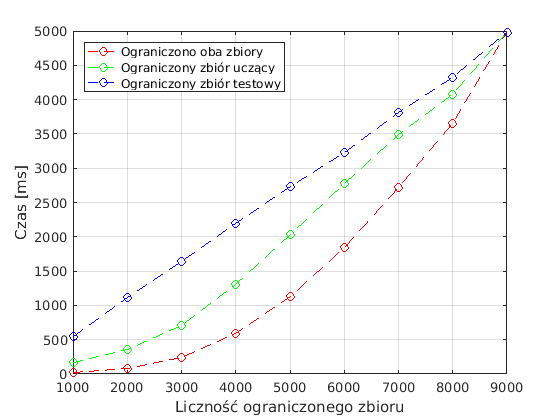
\includegraphics[width=14cm]{img/knn_compexity}
	\caption{Czasowa złożoność obliczeniowa algorytmu $KNN$.}
	\label{fig:knn_compexity}
\end{figure}
\begin{figure}[H]
	\centering
	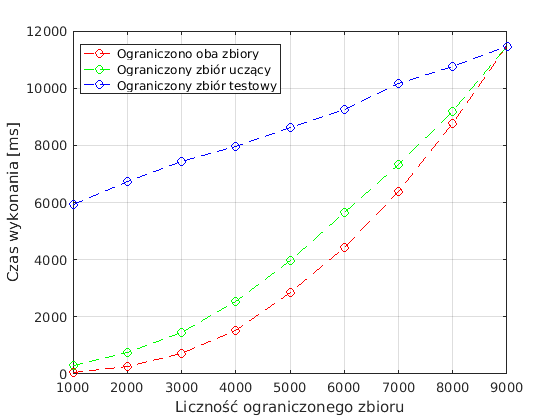
\includegraphics[width=14cm]{img/enn_complexity}
	\caption{Czasowa złożoność obliczeniowa algorytmu $KNN$.}
	\label{fig:enn_complexity}
\end{figure}

W trakcie eksperymentu manipulowano licznością zbioru testowego oraz uczącego. Badano działanie aplikacji dla zmiennej wielkości jednego zbioru przy stałym rozmiarze drugiego równym $9000$ oraz dla zbiorów o takiej samej wielkości w zakresie od $1000$ do $9000$ wektorów. W przypadku obu algorytmów zaobserwować można liniowy wzrost czasu wykonania przy manipulacji rozmiarem jednego zbioru oraz kwadratowy wzrost w przypadku zmiany wielkości obu zbiorów jednocześnie.

Badano możliwość redukcji zbioru uczącego w taki sposób, aby zawierał on taką samą liczbę wektorów dla każdej klasy. Proponowane rozwiązanie pozwala na ograniczenie czasu potrzebnego na przeprowadzenie procesu klasyfikacji, wymaga jednak przygotowania reprezentatywnego zbioru uczącego. Badano możliwość generowania zredukowanego zbioru uczącego przy starcie aplikacji lecz zaobserwowano znaczny spadek skuteczności algorytmów klasyfikacji. 

Zbadano również wpływ wielkości zbioru uczącego na podstawie analizy danych zawierających 32812 wektorów testowych. Wyniki zebrano w tabeli \ref{tab:rozmiar-zbioru-uczacego}.

\begin{table}[H]
	\centering
	\begin{tabular}{|r|r|r|r|r|}
		\hline
		Wielkość zbioru uczącego & Sk. KNN [\%] & Czas KNN [s] & Sk. ENN [\%] & Czas ENN [s]  \\ 
		\hline
		0.1 & 72.82 & 3.066 & 75.93 & 3.950\\
		\hline
		0.2 & 73.18 & 11.754 & 67.52 & 14.505 \\
		\hline
		0.3 & 76.94 & 17.055 & 70.69 & 25.430 \\
		\hline
		0.4 & 80.10 & 19.466 & 74.14 & 34.135 \\
		\hline
		0.5 & 82.24 & 20.552 & 75.75 &  44.992\\
		\hline
		0.6 & 88.80 & 21.104 & 85.01 & 56.602 \\
		\hline
		0.7 & 96.18 & 17.040 & 93.68 & 63.049 \\
		\hline
		0.8 & 95.61 & 14.335 & 92.62 & 78.166 \\
		\hline
		0.9 & 96.34 & 8.333 & 94.14 & 86.396 \\
		\hline
	\end{tabular}
	\caption{Porównanie skuteczności i czasu działania aplikacji dla zbiorów uczących i testowych różnych wielkości.}
	\label{tab:rozmiar-zbioru-uczacego}	
\end{table}
W kolejnych krokach badano działanie obu metod przy użyciu zbioru uczącego zwierającego zdefiniowaną w pierwszej kolumnie tabeli część wszystkich danych. Pozostałe wektory trafiały do zbioru testowego. Zaobserwowano wzrost skuteczności obu algorytmów wraz ze wzrostem wielkości zbioru uczącego do wartości $0.7$. W obu przypadkach nie zauważono znaczących zmian skuteczności dla wartości z zakresu $0.7-0.9$. Na podstawie omawianych danych można stwierdzić, że czas wykonania algorytmu $ENN$ zależy w większym stopniu od rozmiaru zbioru uczącego niż testowego. Wynika to z nietrywialnego procesu uczenia klasyfikatora. W przypadku algorytmu $KNN$ zaobserwowano mniejsze wartości czasu wykonania w końcowej fazie eksperymentu.
\subsection{Wskaźniki jakości klasyfikatora}

Dla uzyskanych wyników klasyfikacji zostały wyznaczone wskaźniki jakości takie jak czułość i swoistość. Czułość określa w tym przypadku zdolność algorytmu do wykrycia choroby, czyli dla czułości równej 1, algorytm potrafi w każdym przypadku poprawnie wykryć chorobę. Swoistość określa zdolność algorytmu do poprawnej klasyfikacji osób zdrowych. Wskaźniki opisują jedynie zdolność klasyfikacji zdrowy/chory, nie bada jednak klasyfikacji pomiędzy poszczególne choroby. 
\newline
Wskaźniki obliczane są według następujących wzorów:

\begin{equation}
czulosc = \frac{Tp}{Tp+Fn}
\end{equation}

\begin{equation}
swoistosc = \frac{Tn}{Tn+Fp}
\end{equation}
\newline
TP – True Positive – liczba obserwacji poprawnie zaklasyfikowanych do klasy pozytywnej
\newline
TN – True Negative – liczba obserwacji poprawnie zaklasyfikowanych do klasy negatywnej
\newline
FP – False Positive – liczba obserwacji zaklasyfikowanych do klasy pozytywnej podczas, gdy w rzeczywistości pochodzą z klasy negatywnej
\newline
FN – False Negative – liczba obserwacji zaklasyfikowanych do klasy negatywnej podczas, gdy w rzeczywistości pochodzą z klasy pozytywnej


Dla niektórych plików obliczenie wskaźników nie było możliwe, ze względu na zerową wartość sumy znajdującej się w mianowniku. Jest to spowodowane m.in występowaniem tylko jednej klasy w niektórych plikach. W takim przypadku wszystkie próbki klasyfikowane są jako występujaca klasa, a skuteczność działania wynosi 100\%.

\begin{table}[H]
	\centering
	\begin{tabular}{|c|r|r|r|r|}
		\hline
		& \multicolumn{2}{c|}{$kNN$} & \multicolumn{2}{c|}{$eNN$} \\
		\hline
		$Plik$ & Czułość & Swoistość & Czułość & Swoistość \\
		\hline
100 &1 &1 &0.85714 &1\\                  
\hline                                   
101 &--- &1 &--- &0.9951\\               
\hline                                   
102 &0.99451 &--- &1 &---\\              
\hline                                   
103 &--- &1 &--- &1\\                    
\hline                                   
104 &0.9625 &0.9375 &0.9625 &0.9375\\    
\hline                                   
105 &0.5 &1 &0.5 &0.99795\\              
\hline                                   
106 &0.96721 &1 &0.96721 &1\\            
\hline                                   
108 &0 &1 &0 &1\\                        
\hline                                   
109 &1 &--- &1 &---\\                    
\hline                                   
111 &1 &--- &1 &---\\                    
\hline                                   
112 &--- &1 &--- &1\\                    
\hline                                   
113 &0 &1 &1 &0.98684\\                  
\hline                                   
118 &1 &--- &1 &---\\                    
\hline                                   
119 &0.86667 &1 &0.86667 &1\\            
\hline                                   
121 &--- &1 &--- &1\\                    
\hline                                   
122 &--- &1 &--- &1\\                    
\hline                                   
124 &1 &--- &1 &---\\                    
\hline                                   
200 &0.5 &1 &1 &0.97059\\                
\hline                                   
201 &0 &1 &0.071429 &1\\                 
\hline                                   
202 &--- &0.99371 &--- &0.93082\\        
\hline                                   
203 &--- &1 &--- &1\\                    
\hline                                   
205 &0 &1 &0 &1\\                        
\hline                                   
208 &0.85 &0.97166 &0.85 &0.92713\\      
\hline                                   
209 &0.44444 &0.98165 &0.88889 &0.9633\\ 
\hline                                   
210 &0 &1 &0 &0.99819\\                  
\hline                                   
212 &1 &1 &1 &1\\                        
\hline                                   
213 &0.77419 &0.98085 &0.80645 &0.94256\\
\hline                                   
214 &1 &--- &1 &---\\                    
\hline                                   
215 &1 &1 &1 &1\\                        
\hline                                   
217 &0.80952 &1 &0.80952 &1\\            
\hline                                   
219 &0 &1 &0 &0.978\\                    
\hline                                   
221 &1 &0.99187 &1 &0.99187\\            
\hline                                   
222 &0.7 &0.90598 &0.86667 &0.81766\\    
\hline                                   
223 &0.90625 &--- &0.90625 &---\\        
\hline                                   
228 &0.95 &1 &0.95 &0.9924\\             
\hline                                   
231 &0.99698 &0.98 &0.99698 &1\\         
\hline                                   
233 &0.85714 &1 &0.85714 &0.99467\\      
\hline                                   
234 &--- &1 &--- &1\\                    
\hline                                   
	\end{tabular}
	\caption{Czułość i swoistość algorytmu kNN i eNN.}
	\label{tab:matlab-wskazniki}
\end{table}
\subsection{Omówienie możliwości wykorzystania zrównoważonego zbioru uczącego?}

\subsection{Rozkład danych w zbiorze uczącym i testowym.}
W rozdziale \ref{chap:prototype} została przedstawiona skuteczność działania algorytmu dla różnych plików. W tym rozdziale zostaną omówione rozkłady klas w niektórych plikach, oraz ich wpływ na działanie algorytmu.


W tabeli \ref{tab:matlab-plik100} został przedstawiony rozkład klas w pliku 100. W pliku występują dwie klasy 1 i 3. Pomimo bardzo dużej różnicy pomiędzy licznością obu klas podczas klasyfikacji za pomocą metody eNN tylko jedna próbka została źle sklasyfikowana, natomiast algorytm kNN był bezbłędny. W tym przypadku 10 próbek z klasy 3 wystarcza do przeprowadzenia poprawnego procesu uczenia algorytmów.

\begin{table}[H]
	\centering
	\begin{tabular}{|c|r|r|r|r|}
		\hline
		
		Klasa & Zbiór uczący & Zbiór testowy & Klasyfikacja kNN & Klasyfikacja eNN \\
		\hline
		1 & 737 & 314 & 314 & 315 \\
		\hline 
		3 & 10 & 7 & 7 & 6 \\
		\hline
                          
	\end{tabular}
	\caption{Szczegółowy rozkład klas dla pliku 100}
	\label{tab:matlab-plik100}
\end{table}

[TODO]

\begin{table}[H]
	\centering
	\begin{tabular}{|c|r|r|r|r|}
		\hline
		
		Klasa & Zbiór uczący & Zbiór testowy & Klasyfikacja kNN & Klasyfikacja eNN \\
		\hline
		1 & 61 & 16 & 18 & 18 \\
		\hline 
		3 & 3 & 0 & 0 & 6 \\
		\hline
		4 & 159 & 80 & 78 & 72 \\
		\hline
		
	\end{tabular}
	\caption{Szczegółowy rozkład klas dla pliku 104}
	\label{tab:matlab-plik104}
\end{table}


W tabeli \ref{tab:matlab-skutecznosc} opisującej skuteczność działania algorytmów zdecydowanie wyróżniają się wyniki uzyskane dla pliku 201. W tabeli \ref{tab:matlab-plik201} został przedstawiony rozkład klas w tym pliku. Niska skuteczność działania algorytmu wynika ze źle przygotowanego zbioru uczącego, w którym nie znalazły się próbki z klas 3 i 7 co uniemożliwiło ich poprawną klasyfikację. Dodatkową przeszkodą była niska liczebność zbioru co wiąże się z małą ilością próbek poszczególnych klas.

\begin{table}[H]
	\centering
	\begin{tabular}{|c|r|r|r|r|}
		\hline
		
		Klasa & Zbiór uczący & Zbiór testowy & Klasyfikacja kNN & Klasyfikacja eNN \\
		\hline
		1 & 66 & 15 & 29 & 28 \\
		\hline 
		3 & 0 & 8 & 0 & 0 \\
		\hline
		4 & 1 & 0 & 0 & 1 \\
		\hline
		7 & 0 & 6 & 0 & 0 \\
		\hline
		
	\end{tabular}
	\caption{Szczegółowy rozkład klas dla pliku 201}
	\label{tab:matlab-plik201}
\end{table}





\section*{Podsumowanie}

W ramach projektu zaproponowano klasyfikatory sygnału $EKG$ opierające się na metodach $KNN$ i $ENN$. Zbudowano prototypy algorytmów w języku $Matlab$ a następnie zaprojektowano kompatybilną z prototypami aplikację w języku $C++$. Przeniesienie części algorytmicznej było możliwe dzięki wykorzystaniu bibliotek wspierających obliczenia na wektorach i macierzach. 
Przeprowadzono szereg testów mających na celu zbadanie skuteczności działania algorytmów oraz wyznaczono wskaźniki czułości i swoistości klasyfikatorów. Na podstawie uzyskanych wyników przyjęto większą użyteczność klasyfikatora $KNN$ w omawianym zadaniu. Średnia skuteczność jest wyższa o kilka punktów procentowych względem $ENN$ przy kilkukrotnie niższej złożoności czasowej aplikacji. Algorytm $ENN$ pozwolił jednak na zwiększenie skuteczności klasyfikacji w przypadku klas o niewielkiej liczności w zbiorze uczącym. \textbf{jeszcze jakieś zalety?}
Badane metody klasyfikacji mogą pracować równolegle na jednym zbiorze uczącym, co pozwala na wykorzystanie technik programowania na systemy wieloprocesorowe. Wykorzystany w ramach projektu interfejs $OpenMP$ pozwolił na kilkukrotne zmniejszenie czasu potrzebnego na analizę zbioru testowego względem aplikacji jednowątkowej. Dalszą poprawę wydajności mogłoby dać wykorzystanie biblioteki $OpenCL$ lub pokrewnej.

\begin{thebibliography}{9}
	\bibitem{haibo-he} 
	Bo Tang i Haibo He. 
	\textit{Enn: Extended Nearest Neighbor Method for Pattern Recognition}. 
	IEEE Computational intelligence magazine. 2015
	
	\bibitem{enn-impl}
	Haibo He.
	\textit{Referencyjna implementacja algorytmu eNN}.
	\\\texttt{http://www.ele.uri.edu/faculty/he/research/ENN/ENN.html}
	
	\bibitem{qrs-wiki}
	Wikipedia.
	\textit{QRS complex}.	\\\texttt{https://en.wikipedia.org/wiki/QRS\_complex}
	
	\bibitem{knn-wiki}
	Wikipedia.
	\textit{k-nearest neighbors algorithm}.	\\\texttt{https://en.wikipedia.org/wiki/K-nearest\_neighbors\_algorithm}
	\bibitem{mitdb}
	\textit{MIT-BIH Arrhythmia Database}.	\\\texttt{https://www.physionet.org/physiobank/database/mitdb/}
	
	\bibitem{heart-class-module} 
	Michał Ciszewski, Łukasz Dudek i Krystian Mucha.
	\textit{Moduł HeartClass}.
	
	\bibitem{eigen-www}
	\textit{Eigen Library}.
	\\\texttt{http://http://eigen.tuxfamily.org/}
\end{thebibliography}


\begin{appendices}
\section{Struktura projektu}
Repozytorium projektu podzielone jest na szereg katalogów.
\begin{itemize}  
	\item cpp - kod źródłowy programu w języku C++ 
	\item data - zbiór danych testowych wraz z plikami definiującymi klasy
	\item doc - wykorzystane artykuły naukowe
	\item matlab - kod źródłowy prototypu w języku Matlab
	\item raport - raport podsumowujący projekt
	\item util - wykorzystane narzędzia pomocnicze
\end{itemize}


Zalecana metoda kompilacji wymaga wykonania następujących poleceń:
\begin{lstlisting}[language=bash,caption=Kompilacja programu]
git clone --recursive https://github.com/wgml/ecg-classification.git
cd ecg-classification
mkdir build
cd build
cmake ../cpp/knn-ecg
make
\end{lstlisting}

W trakcie klonowania zawartości repozytorium pobierane są również zależności projektu. Kompilacja wymaga kompilatora wspierającego standard $c++11$, a cały proces testowany był przy użyciu zbioru kompilatorów $GCC$ w wersji $6.2.1$. Aplikacja wykorzystuje interfejs $OpenMP$. W przypadku niedostępności tej biblioteki w systemie, konieczne jest zmodyfikowanie pliku $cpp/knn-ecg/CMakeLists.txt$ i usunięcie argumentu $-fopenmp$ z listy flag kompilatora.

W wyniku kompilacji powstają dwa pliki źródłowe - $knn$ oraz $enn$.
Uruchomienie klasyfikatora wymaga przekazania ścieżek do katalogów testowych przez argumenty wiersza poleceń. Poniżej przedstawiono przykładowe wywołania.

\begin{lstlisting}[language=bash,caption=Uruchamianie aplikacji]
./knn ../data/data_unique_labels/101 ../data/data_unique_labels/102
./enn ../data/data_unique_labels/*
\end{lstlisting}

Domyślnie aplikacja wykorzystuje wspólne pliki danych dla zbioru testowego i uczącego i dzieli jest w stosunku 7 do 3. W celu wykorzystania dwóch plików wejściowych koniecznie jest przekazanie argumentu $--multi-data-file$.
Wynik działania programu przedstawiany jest w formie tekstowej w konsoli terminala.

Poprawność działania prototypowej wersji potwierdzony przy użyciu programu $Matlab$ w wersji $R2016b$. Udostepniono plik źródłowy $knn_vs_enn.m$ odpowiedzialny za przeprowadzenie procesu uczenie i testowania na zbiorze plików oraz wyznaczenie wskaźników opisujących klasyfikatory.

Pomocnicze skrypty napisane zostały przy użyciu języków $Python 3$ oraz $Bash 4$.
\end{appendices}



%%}
\end{document}
